% --- Grounding DINO and DINOv2 ---
% --- Detection: Grounding DINO ---
\begin{frame}{Detection Foundation Model: Grounding DINO}
  \begin{itemize}
    \item Open-vocabulary detection with natural-language grounding.
    \item Uses transformer-based backbone for both image and text encoding.
    \item Matches object proposals in an image with user-provided text prompts (e.g. "a red backpack").
    \item Produces bounding boxes, labels, and confidence scores for detected objects.
    \item \textbf{Key architectural mechanisms}:
      \begin{itemize}
        \item \textbf{Feature enhancer neck} with deep image-text cross-attention (not only late fusion).
        \item \textbf{Language-guided query selection} to initialize decoder queries on relevant regions.
        \item \textbf{Cross-modality decoder head} for iterative region-text refinement.
      \end{itemize}
    \item \textbf{Takeaway:} strong transfer to unseen categories and prompts.
  \end{itemize}
\end{frame}

\begin{frame}{Grounding DINO: How It Works}
  \centering
  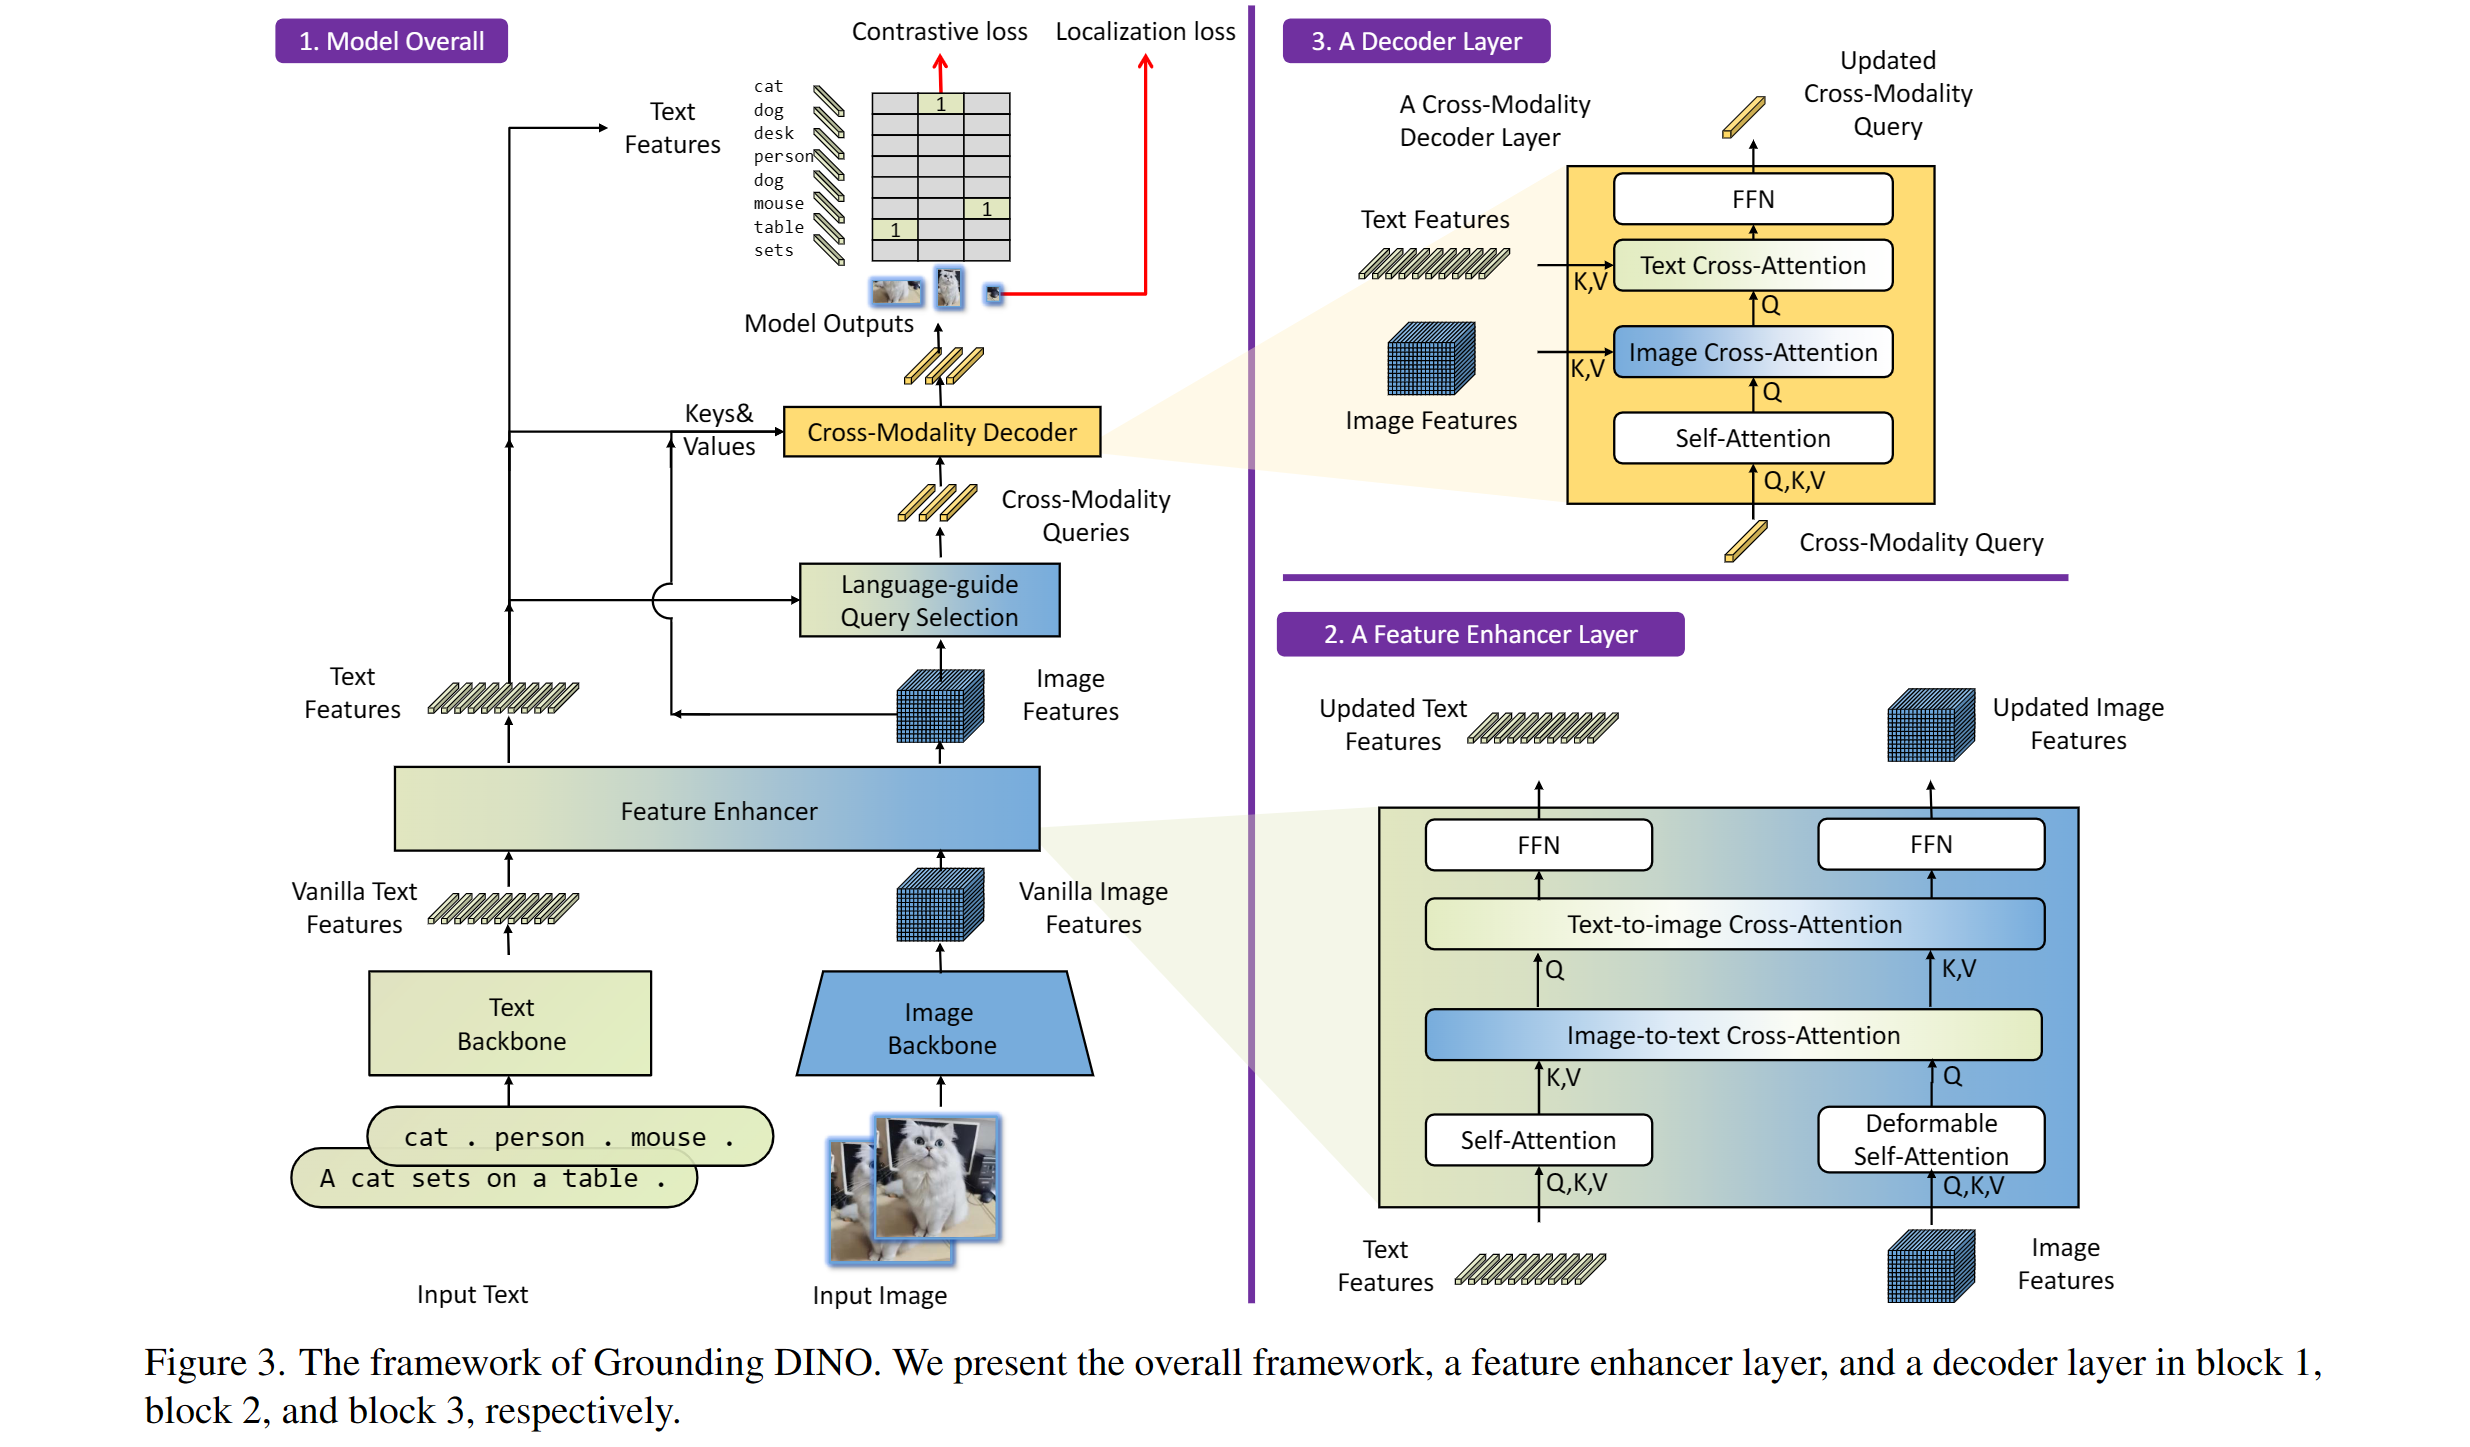
\includegraphics[width=0.8\textwidth]{assets/New-Lecture_Foundation_models/grounding_dino_example.png}
\end{frame}

\begin{frame}{DINOv2: Transformer-based representation learner
  trained on 142 million images}
  \centering
  
\includegraphics[width=\textwidth,height=0.86\textheight,keepaspectratio]{assets/New-Lecture_Foundation_models/stanford_biods276_lecture1/slide_25.png}
\end{frame}

\begin{frame}{DINOv2: Transformer-based representation learner
  trained on 142 million images}
  \centering
  
\includegraphics[width=\textwidth,height=0.86\textheight,keepaspectratio]{assets/New-Lecture_Foundation_models/stanford_biods276_lecture1/slide_26.png}
\end{frame}
